% \begin{preamble}
\documentclass[12pt]{article}
\usepackage[margin=1in]{geometry}
\usepackage[utf8]{inputenc}
\renewcommand{\rmdefault}{phv} % Arial Font
\renewcommand{\sfdefault}{phv} % Arial Font
\usepackage{color}
\usepackage{tcolorbox}
\usepackage{graphicx}
\usepackage{ragged2e}
\graphicspath{ {./figures/}} % Location of the graphics files
\usepackage[labelfont=bf]{caption}
\usepackage{multicol}
\usepackage{nopageno} % remove page numbers
\pagestyle{empty} % remove page numbers
\usepackage{gb4e}
\noautomath
% \end{preamble}

\newcommand{\glr}{\textcolor{teal}}
\definecolor{Purple}{RGB}{255,10,140}
\newcommand{\jd}[1]{\textcolor{Purple}{[jd: #1]}}
\newcommand{\mm}[1]{\textcolor{teal}{[mm: #1]}}

% Modify sections so they appear as normal text
\usepackage{titlesec}  % Allows customization of section formatting
\titleformat{\section} % Redefine section format
  [runin]  % Makes section title run into the paragraph
  {\normalfont\bfseries}  % Bold, normal font
  {}  % No section number
  {0pt}  % No space before text
  {}  % No special formatting after title

\titlespacing*{\section}{0pt}{0pt}{0pt}  % Remove all spacing


% To insert wordcount (but you can't use overleaf for this)
% This is easier to use with the section code above
% Run in the command line:
% texcount -sub=section main.tex | awk '/Introduction/,/Discussion/ {getline; print $0}' | awk '{sum+=$1} END {print sum}' > wordcount.txt
% pdflatex main.tex

\immediate\write18{texcount -sum -inc -q main.tex > wordcount.txt}
\newcommand{\insertwordcount}{%
    \input{wordcount.txt}%
}


\begin{document}
% Title
\centerline{\textbf{Affective X conceptual information in the battle of linguistic meaning}}
% \centerline{Morgan Moyer, Anouch Bourmayan (Sorbonne University), Isidora Stojanovic and Brent Strickland (Jean-Nicod, ENS-PSL/CNRS}
% \centerline{mcmoyer11@gmail.com}%names
% Endtitle 
\centerline{Word Count: 764}
\normalsize
\bigskip


\section{Introduction}. 
If someone on the street yelled ``Hey f*ck you!'' you would feel quite flummoxed and not a little emotional. For expletive expressions, the negative valence is a core component of their meaning. Words also have a dimension of meaning that can be described as Conceptual: the verb `love' is generally considered as having a positive valence, but also generally describes a psychological/abstract event or state of being. In contrast, `hug', while also of positive valence, more describes a physical/concrete event or state of being. The \textbf{ Affect-First Hypothesis} (AFH) is the psychological hypothesis that affective information is processed before conceptual information [1,2]. In the domain of word meaning and the lexicon, it would predict that affective is accessed prior to conceptual meaning. Concretely, judgments of a word's valence (positive or negative value) should be made faster than judgements of a word's conceptual feature(s). This appears true for expletives/slurs, whose affective meaning often triggers a physiological response (``hot'' affect). Does it hold for `love'/`hug' where a positive judgement probably doesn't entail an elevated heart rate or sweaty palms (``cold'' affect)? We present several experiments providing evidence that 'yes', supporting the AFH. We ask:

% \vspace{-.3cm}
\begin{tcolorbox}[colback=white]
% \vspace{-.2cm}
\centering
\textbf{Q1 (specific)}: Are valence judgments cognitively prior to conceptual judgments? \\ 
\textbf{Q2 (specific)}: Do lexical categories (and eventually words) pattern differently?\\
\textbf{Q3 (broad)}: How do conceptual dimensions relate to core categories?
% \vspace{-.2cm}
\end{tcolorbox}
% \vspace{-.2cm}

\section{Background}.
% \mm{The last 20 years have seen a rise in the study of not-strictly-truth-conditional aspects of meaning which had previously been sidelined from linguistic analysis in Fregean traditions.} 
Affective meaning forms a natural class with slurs, expressivity, and evaluativity, and was traditionally dismissed as a secondary dimension in semantic analysis [3-9], although recently this view has been challenged [ibid.] and affect has also been found to aid the hearer in anticipating the speaker's referential intentions [10]. Neuroscientific research has shown mixed evidence for AFH, or ``affect effects'' [11-15], but has recently acknowledged the role of contextual information, %in the modulation of affect effects, 
for example, Task effects [15,16] and the communicative situation [17a]. 


One challenge to testing AFH is targeting an appropriate conceptual dimension for comparison with affect, because words vary greatly on which conceptual dimension(s) best track(s) meaning [18a-21]. We compare valence to four different dimensions of conceptual information chosen for their foundational role in core cognition. First, the dimension of \textbf{physical vs. psychological} (Exp1) (e.g., [21a,21b]), 
then \textbf{abstract vs. concrete} (Exp2) (e.g., [20])), and finally \textbf{animate vs. inanimate} (Exp3) (e.g., [21c]). These categories were chosen based on their relation to theories of core meaning, as well. Finally, we test valence against syntactic category judgments (nouns vs. verbs). Although syntactic information is not conceptual (perhpas in the same way), this information is argued to be retrieved early [21d], we thus hypothesized that it would serve as a better foil to test the AFH. To preview our results, we found Affect Effects for all except Animacy, which we argue is due to animacy's priviledged role in development and cognition.


\section{Methodology: Speeded Categorization Task}. A binary-forced choice task where participants categorize single words shown alone on a screen one after the other, as quickly as possible. We measure Reaction Time and Response (/Accuracy). We tested Valence against 4 different foils: Exp1 (Verbs, n=12) used physical/psychological response choices, Exp2 (Nouns n=20, Verbs n=20, Adjectives n=20), used concrete/abstract, Exp3 (nouns, n=20) used animate/innimacy, and Exp4 (Nouns and Verbs, n=20) tested syntactic category. \textbf{Stimuli Selection}: each word list had 10 words from each combination of Valence and Conceptual features. Words were chosen either from pilot data, prior norming studies ([22,23]), finally using AI tools or intuition where no prior norms existed. From norming data, we either maximized or minimized mean rating for the target dimension value, and always minimized rating variance. For each experiment 40 word were selected from these norms to represent the best of each combination of feature values (4 total, positive/negative valence x +/-conceptual feature) to reduce uncertainty about word meaning as a potential confound on Reaction Time. Since not all words match on the different dimensions, the experiments did not use the same 40 words.


\section{Results: Reaction Time}. For ease of presentation, we present all the results together. Analyses used mixed effects models, with the biggest RE structure justified by design.  LogRTs for Valence categorization were faster than Conceptual categorization (Affect Effect) for Phys vs. Psych (verbs: $p<$.0005), Conc vs. Abs (Verbs: p$<$.0003, Nouns: p$<$.0003, Adjs. p$<$.0005), and Sytnactic judgements (nouns vs. verbs, p$<$.0005). Only for Ani vs. Inani was there no Affect effects (p=.14). There was no interaction with Lexical Category, but mean RTs revealed Nouns were fastest (Valence: M=741, sd=294; Concrete: M=880, sd=409), followed by Adjs (Val: M=793, sd=347; Conc: M=962, sd=469), and then Verbs (Val: M=860, sd=379; Conc: M=1003, sd=488).

\section{Results: Accuracy}.
It's possible that our RT effects were driven by low accuracy on the Conceptual dimension, consistent with long discussion on conceptual dimensions (e.e., [20]). Unsurprisingly, we found interactions with Accuracy: uncertainly about a word's meaning (ambiguity) results in an elongated RT in a forced-choice task. We looked at items in Exp2 with highest Accuracy on Conc/Abs (for each category). We asked (1) was there still an effect of Task? (2) was there an interaction with Accuracy? Answers: 'Yes' (p$<$.0002), and 'No' (p$>$.27). While accuracy certainly played a role overall, Affect Effects persisted when conceptual meaning is unambiguous.


\section{Discussion}.
We found Valence RTs were faster than Conceptual RTs for 3/4 dimensions (Q1). This is compelling evidence for AFH and the importance of affect for word meaning. While poor Accuracy did increase RTs in the Conceptual Task (ambiguisty leads to increased RT), high accuracy words still maintained faster RTs on the Valence Task. Additionally, all syntactic categories revealed Affect Effects (Q2) for the Concreteness dimension, which we were able to test with Verbs, Nouns and Adjectives. Overall, Nouns were fastest (), followed by Adjectives, then Verbs (). Nouns were also exceptional because of Animacy, which doesn't apply to Verbs/Adjs simply, revealing that all conceptual categories are not created equal (Q3). Animacy judgments were as fast as Valence (nonetheless mean RTs were slower, Ani: M=791ms, sd=321, Val: M=752ms, sd=279). Animacy, like Valence, is paramount in development and thus core cognition [21c]. AFH does not hold monolithically over all conceptual dimensions, nor over the lexicon. Lexical variability in affect effects revealed clusters based on e.g., the centrality of affect to core meaning: while 'love' or 'f*ck' show it, 'sandwich' does not (despite a high positive rating).


% ghost lines to reserve space for author names
\centerline{}

\newpage
\footnotesize

%%%%%%%%%%%%%%%%%%%%%%%%%%%%%%%%%%%%%%%%
% First Row
%%%%%%%%%%%%%%%%%%%%%%%%%%%%%%%%%%%%%%%%
\noindent
\begin{minipage}{0.5\linewidth}
\begin{tcolorbox}[colback=white]
    \hspace*{-.3cm}
    \vspace{-.5cm}
    % \centering
    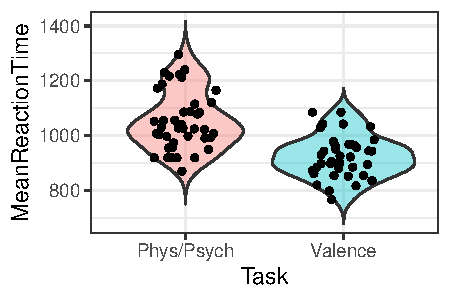
\includegraphics[scale=0.9]{figures/exp1.pdf}
    % \vspace{.2cm}
    \centering
    \captionof{figure}{\footnotesize Exp1: Affect Effect for Phys/Psych ($\beta$=-.13, SE=.03,t=-4.53, p$<$.0005.)}
    \label{fig:exp1}
\end{tcolorbox}
\end{minipage}
\hfill
\begin{minipage}{0.48\linewidth}
    \begin{tcolorbox}[colback=white]
    \hspace*{-.3cm}
    \vspace{-.5cm}
    \centering
    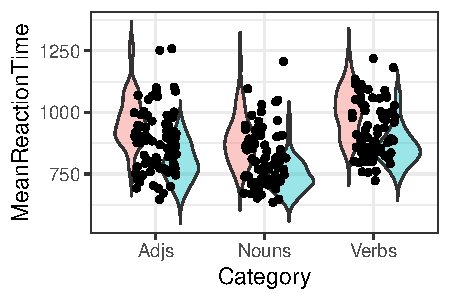
\includegraphics[scale=.9]{figures/exp2_category.pdf}
    % 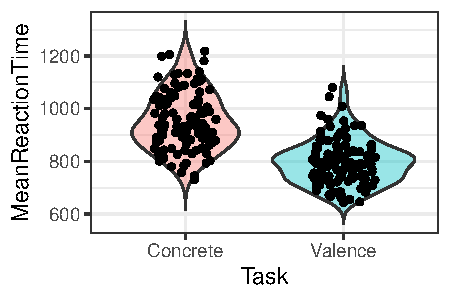
\includegraphics[scale=0.9]{figures/exp2.pdf}
    % \vspace{-.1cm}
    \captionof{figure}{\footnotesize Exp2: Affect Effect for Conc/Abs ($\beta$=-.15, SE=.02, t=-7.34, p$<$.0005).}

    \label{fig:exp2}
    % \vspace{-.2cm}
    \end{tcolorbox}
\end{minipage}


%%%%%%%%%%%%%%%%%%%%%%%%%%%%%%%%%%%%%%%%
% Second Row
%%%%%%%%%%%%%%%%%%%%%%%%%%%%%%%%%%%%%%%%
\noindent
\begin{minipage}{0.5\linewidth}
\begin{tcolorbox}[colback=white]
    \hspace*{-.3cm}
    \vspace{-.5cm}
    % \centering
    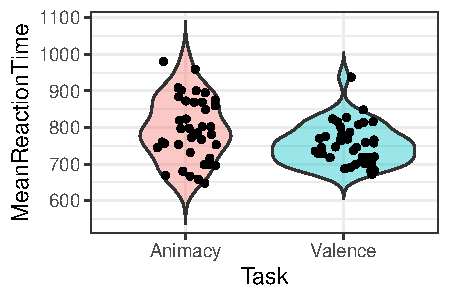
\includegraphics[scale=.9]{figures/exp3.pdf}
    % \vspace{.2cm}
    \centering
    \captionof{figure}{\footnotesize Exp3: No Affect Effect for Animacy ($\beta$=-.04, SE=.03, t=-1.53, p=.14).}
    \label{fig:exp1}
\end{tcolorbox}
\end{minipage}
\hfill
\begin{minipage}{0.48\linewidth}
    \begin{tcolorbox}[colback=white]
    \hspace*{-.3cm}
    \vspace{-.5cm}
    \centering
    % 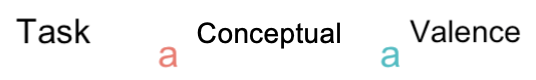
\includegraphics[scale=0.6]{figures/legend.png}
    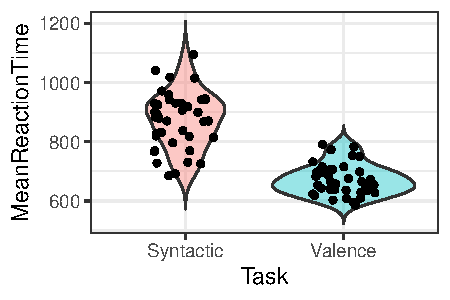
\includegraphics[scale=.9]{figures/exp4.pdf}
    % \vspace{-.75cm}
    \captionof{figure}{\footnotesize Exp4 : Affect Effect for Syntactic ($\beta$=-.24, SE=.04, t=-6.55, p$<$.0005).}
    \label{fig:exp2}
    % \vspace{-.2cm}
    \end{tcolorbox}
\end{minipage}

%%%%%%%%%%%%%%%%%%%%%%%%%%%%%%%%%%%%%%%%
% Third Row
%%%%%%%%%%%%%%%%%%%%%%%%%%%%%%%%%%%%%%%%

\vspace{.2cm}

\noindent
\begin{tcolorbox}[colback=white]
\begin{minipage}{0.7\linewidth} 
    \vspace{-.3cm}
    \hspace{-.5cm}
    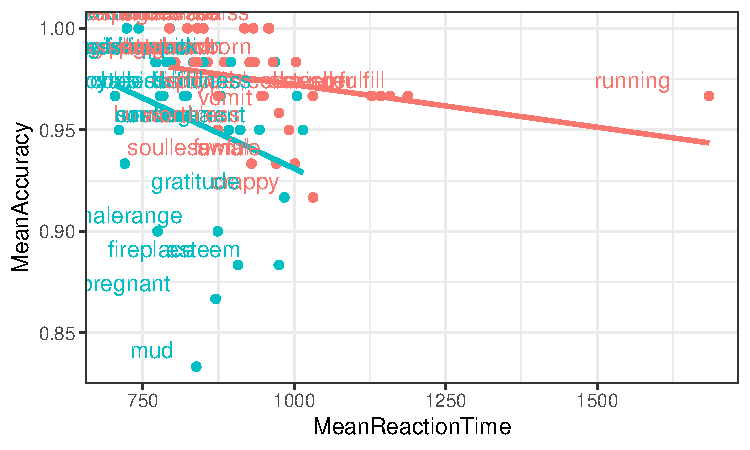
\includegraphics[scale=0.7]{figures/ConcAbs_accXrt.pdf}
    \vspace{-.2cm}
    % \hspace{1cm}
\end{minipage}
\hspace{-2cm}
\begin{minipage}{0.4\linewidth} 
% \centering
    % \hspace{-1cm} 
    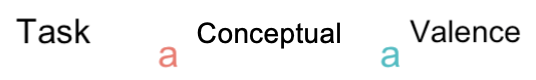
\includegraphics[scale=0.5]{figures/legend.png}
    % \hrule
    % \vspace{.3cm}
    \centering
    \captionof{figure}{\footnotesize From Exp2, the 30 words with highest acceracy on Conceptual Task per lexical category. No Task X Accuracy interaction on RT ($\beta$=-0.07, SE=.06, t=-1.2, p=.27). No main effect of Acuracy ($\beta$=-.03, SE=.03, t=-.88, p=.4), but significant effect of Task ($\beta$=-.11, SE=.3, t=-4.03, p$<$.0002). }
    \label{fig:exp2-items}
    \hspace{-1cm}
\end{minipage}
\end{tcolorbox}


%%%%%%%%%%%%%%%%%%%%%%%%%%%%%%%%%%%%%%%%
% References
%%%%%%%%%%%%%%%%%%%%%%%%%%%%%%%%%%%%%%%%

\footnotesize
\noindent \textbf{References}.
[1] Wundt 1907
[2] Zajonc 1980, 2000
[3] Potts 2005 
[4] Schlenker 2007 
[5] Kaplan 1999 
[6] McCready 2010, 2020 
[7] Gutzmann 2015 
[8] Stojanovic \& Kaiser 2023 
[9] Stojanovic in press 
[10] Ronderos \& Domaneschi 2023 
[11] Storbeck \& Robinson 2004 
[12] Storbeck \& Clore 2007 
[13] Nummenmaa, Hyönä \& Calvo 2011 
[14] Rohr \& Wentura 2023 
[15] Hinojosa, Moreno \& Ferré 2019 
[16] Hinojosa, Herbert, \& Kissler 2023
[17a] Rohr \& Abdel Rahman 2015 
[17] Levin 1993
[18] Kousta, Vigliocco, Vinson, Andrews and Del Campo 2011 
[19] Lynott, Connell, Brysbaert, Brand \& Carney 2019 
[20] Vigliocco, Kousta, Della Rosa, Vinson, Tettamanti, Devlin 2014 
[21] Winter 2022 
[22] Herbert 2023 
[23] Strickland, Silver, \& Keil 2017
[24] Kuhn, Geraci, Schlenker \& Strickland 2021
[25] Opfer \& Gelman 2011
[26] Strijkers \& Costa 2011
[27] Warriner, Kuperman \& Brysbaert 2013
[28] Brysbaert, Warriner \& Kuperman 2013

\end{document}


